\documentclass[11pt, oneside, a4paper, fleqn]{article}
%Auch als report nutzbar
%fleqn= flush left equation
% use "amsart" instead of "article" for AMSLaTeX format
\usepackage[top=1cm]{geometry}
\geometry{a4paper, lmargin=25mm, rmargin=25mm, tmargin=25mm, bmargin=25mm} 

\usepackage[onehalfspacing]{setspace}   	

%\usepackage[parfill]{parskip}
% Activate to begin paragraphs with an empty line rather than  anindent

\usepackage[dvipsnames]{xcolor}
\usepackage[ngerman]{babel}
\usepackage[latin1]{inputenc}
\usepackage{amssymb}
\usepackage{amsmath}
\setlength\mathindent{0pt}
%\usepackage{chemfig}
\usepackage{graphicx}
\usepackage{tabularx}	
\usepackage{tikz}
\usetikzlibrary{arrows,automata,shapes,positioning}
\usepackage[T1]{fontenc}
\usepackage{float}
\usepackage{color}
\usepackage{listings}
\lstset{basicstyle=\footnotesize\ttfamily,breaklines=true}
\usepackage{courier}
\parindent0pt
\newcommand{\red}[1]{\textcolor{Red}{#1}}
\newcommand{\gr}[1]{\textcolor{Green}{#1}}
\newcommand{\tab}{\hspace*{5mm}}
\newcommand{\gf}[1]{\dq{#1}\dq{}}
\newcommand{\RM}[1]{\MakeUppercase{\romannumeral #1{}}}
\newcommand{\hl}[1]{\textit{\textcolor{red}{#1}}}


\title{\vspace*{-10mm} Datenbanksysteme SoSe 18\\�bung 2}
\author{Gruppe 90, Dienstag 16-18h bei Alexander Schulz:\\Mara Steiger, Jonas von der Heyden, Alia Rothkegel}
\date{}


\begin{document}
\lstset{language=bash} 
\maketitle
\section{Grundlagen}
\subsection{Geben Sie im ER-Modell ein Beispiel f�r einen Entit�tstypen mit genau einem Attribut an.}

\begin{figure}[!h]
\centering
\begin{tikzpicture}%[->,>=stealth', node distance=2.8cm, semithick]
\tikzstyle{entity}=[draw, shape=rectangle, minimum height=1cm, minimum width=2cm]
\tikzstyle{attribute}=[draw, shape=ellipse, minimum height=1cm, minimum width=2cm]
\tikzstyle{relation}=[draw, shape=diamond, minimum width=5cm, minimum height=1cm]
\node[entity] (0) {PROJEKT};
\node[attribute] (1) [right=1.5cm of 0]{\centering \underline{Name}};
%\node[rectangly] (5) [below right=.375cm and 1.5cm of 1]{\centering Diskretisierungsfehler,\\Approximationsfehler,...};
%\node[rectangly] (6) [below right=.375cm and 1.5cm of 2]{\centering Rundungsfehler};

\draw[thick] (0.east) to (1.west);
%\draw[thick] (1.east) to [bend left=45] (2.east);
%\draw[thick] (2.east) to [bend left=45] (3.east);

\end{tikzpicture}
\end{figure}

\subsection{Geben Sie im ER-Modell ein Beispiel f�r eine nicht-rekursive 1-zu-N Relation an.}

\begin{figure}[!h]
\centering
\begin{tikzpicture}%[->,>=stealth', node distance=2.8cm, semithick]
\tikzstyle{entity}=[draw, shape=rectangle, minimum height=1cm, minimum width=2cm]
\tikzstyle{attribute}=[draw, shape=ellipse, minimum height=1cm, minimum width=2cm]
\tikzstyle{relation}=[draw, shape=diamond, aspect=2, inner sep=0pt]
\node[entity] (0) {PERSON};
\node[relation] (1) [right=1.5cm of 0]{\centering gemeldet in};
\node[entity] (2) [right= 1.5cm of 1]{\centering WOHNUNG};
%\node[rectangly] (6) [below right=.375cm and 1.5cm of 2]{\centering Rundungsfehler};

\draw[thick] (0.east) node[anchor=south west] {1} to (1.west);
\draw[thick] (1.east) to (2.west) node[anchor=south east] {N};
%\draw[thick] (2.east) to [bend left=45] (3.east);

\end{tikzpicture}
\end{figure}

\subsection{Geben Sie im ER-Modell ein Beispiel f�r eine nicht-rekursive N-zu-M Relation an.}

\begin{figure}[!h]
\centering
\begin{tikzpicture}%[->,>=stealth', node distance=2.8cm, semithick]
\tikzstyle{entity}=[draw, shape=rectangle, minimum height=1cm, minimum width=2cm]
\tikzstyle{attribute}=[draw, shape=ellipse, minimum height=1cm, minimum width=2cm]
\tikzstyle{relation}=[draw, shape=diamond, aspect=2, inner sep=0pt]
\node[entity] (0) {PERSON};
\node[relation] (1) [right=1.5cm of 0]{\centering belegt};
\node[entity] (2) [right= 1.5cm of 1]{\centering MODUL};
%\node[rectangly] (6) [below right=.375cm and 1.5cm of 2]{\centering Rundungsfehler};

\draw[thick] (0.east) node[anchor=south west] {M} to (1.west);
\draw[thick] (1.east) to (2.west) node[anchor=south east] {N};
%\draw[thick] (2.east) to [bend left=45] (3.east);

\end{tikzpicture}
\end{figure}

\subsection{Geben Sie im ER-Modell ein Beispiel f�r eine rekursive Relation an. Wie sieht es mit dem Kardinalit�tsverh�ltnis Ihres Beispiels aus?}

\begin{figure}[!h]
\centering
\begin{tikzpicture}%[->,>=stealth', node distance=2.8cm, semithick]
\tikzstyle{entity}=[draw, shape=rectangle, minimum height=1cm, minimum width=2cm]
\tikzstyle{attribute}=[draw, shape=ellipse, minimum height=1cm, minimum width=2cm]
\tikzstyle{relation}=[draw, shape=diamond, aspect=2, inner sep=0pt]
\node[entity] (0) {PERSON};
\node[relation] (1) [right=1.5cm of 0]{\centering Geschwister von};
%\node[rectangly] (6) [below right=.375cm and 1.5cm of 2]{\centering Rundungsfehler};

\draw[thick] (0.north) [bend left=30] node[anchor=south east] {N} to (1.north);
\draw[thick] (1.south) [bend left=30] to (0.south) node[anchor=north east] {M};
%\draw[thick] (2.east) to [bend left=45] (3.east);

\end{tikzpicture}
\end{figure}


\section{ER-Modellierung}
\subsection{Erkl�ren Sie den Unterschied zwischen totaler und partieller Partizipation.}
\textbf{Totale Partizipation:} \\
Jede Instanz einer Entit�t der ersten Klasse muss mit einer Instanz der Entit�t der zweiten Klasse in Relation stehen. \\
\textbf{Partielle Partizipation:} \\
Eine Instanz einer Entit�t  kann(!) in Relation zu einer Instanz der zweiten Klasse stehen.

\subsection{Erstellen Sie ein ER-Modell in einfacher Notation auf Grundlage der folgenden Beschreibung. \\
Versuchen Sie sich so nah wie m�glich an die Beschreibung zu halten. \\
Beachten Sie bei der Modellierung die Aspekte der totalen und partiellen Abh�ngigkeit.}
\textbf{Beschreibung:}\\
�rzte behandeln Patienten. �rzte haben einen Namen und eine Spezialisierung. Patienten haben einen Namen, eine Versicherungsnummer und leiden an mehreren Krankheiten. Eine Krankheit wird eindeutig durch einen Namen beschrieben. �rzte d�rfen sich nicht selbst behandeln. Patienten tauschen sich mit anderen Patienten �ber ihre Krankheiten aus. �rzte forschen daran Krankheiten besser heilen zu k�nnen. \\

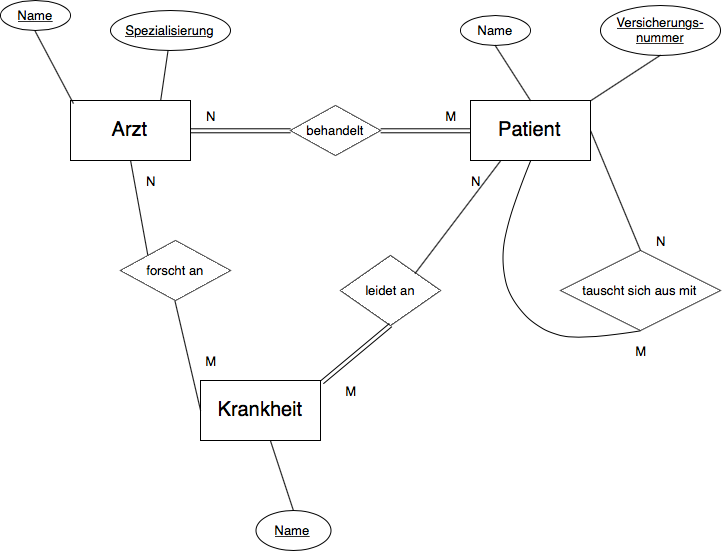
\includegraphics[scale=0.4]{ER1.png}


\subsection{Erstellen Sie ein ER-Modell in Min-Max Notation auf Grundlage der folgenden Beschreibung. Versuchen Sie sich so nah wie m�glich an die Beschreibung zu halten.}
\textbf{Beschreibung:} \\
Menschen werden krank und k�nnen sich gegenseitig anstecken. Ein Patient hat einen Namen, ein Krankheitsbild und eine Privatadresse. Patienten besuchen �rzte an einem bestimmten Tag. Wenn ein Arzt Patient ist, darf er sich nicht selbst besuchen. Ein Arzt hat einen Namen, eine Spezialisierung, eine Privatadresse und eine Dienstadresse. Die Privatadresse eines Arztes liegt immer in der selben Stadt wie die Dienstadresse. 

\section{Webserver \& JavaScript}
\subsection{Installieren sie einen Webserver ihrer Wahl (zum Beispiel einen Apache HTTPD Webserver). Konfigurieren sie ihren Webserver so, dass er unter http://www.localhost:8050 (lokal) erreichbar ist.	Deployen sie unten stehende Webseite (Source Code 1) als index.html in ihren Webserver.}

Anleitung f�r Ubuntu 16.04:
\begin{enumerate}
	\item {\lstinline[basicstyle=\ttfamily]|sudo apt install apache2|}
	\item Port in /etc/apache2/ports.conf zu 8050 �ndern
	\item Port in /etc/apache2/sites-enabled/000-default.conf zu *:8050 �ndern
	\item index.html in /var/www/html/ ersetzen
	\item apache2 starten: {\lstinline[basicstyle=\ttfamily]|service apache2 start|}
\end{enumerate}

\subsection{Schreiben sie eine Javascript-Funktion, die im div Element bereich den Text "Hallo ", erg�nzt	durch den Text aus dem Eingabefeld feld ausgibt, sobald der Knopf knopf gedr�ckt wird. Wenn kein Text im Eingabefeld feld steht soll "Hallo Unbekannter!" im div Element bereich ausgegeben werden}

\lstinputlisting[language=HTML]{server/index.html}

\end{document}
